% ********** Chapter 4 **********
\chapter{AVL-boom}
\label{sec:Hoofdstuk 4}

\begin{figure}[h]
	\centering
		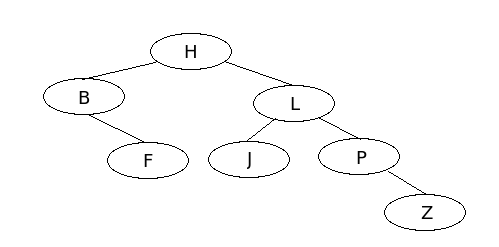
\includegraphics[width=\textwidth]{chap4/avltree}
	\label{fig:avltree}
\end{figure}

\section{Introductie}
De AVL-boom is de eerste gebalanceerde boom die we gaan behandelen. Deze boom lijkt erg veel op de binary boom, alleen heeft de AVL-boom een extra eigenschap, namelijk dat voor elke interne knoop geldt dat de hoogte van de kinderen verschilt met maximaal 1.\\
\\
\section{Zoeken}
Het zoeken gaat op dezelfde manier als bij de binaire boom die behandeld is in hoofdstuk 2.\\
\\
\section{Toevoegen}


% ********** End of chapter **********